\documentclass[../main.tex]{subfiles}
\begin{document}
\chapter{I-measure for Markov chains}
If $X_1\to X_2\to\dots\to X_n$ form a Markov chain, then structure of $\mu^*$ becomes much simpler and the information diagram can be simplified.\\
For example, for $n=3$, $X_1\to X_2\to X_3$ iff $I(X_1;X_3|X_2)=\mu^*(\Tilde{X_1}\cap\Tilde{X_3}-\Tilde{X_2}) =0. $
Therefore, the atom $\Tilde{X_1}\cap\Tilde{X_3}-\Tilde{X_2}$ can be neglected in the information diagram.

 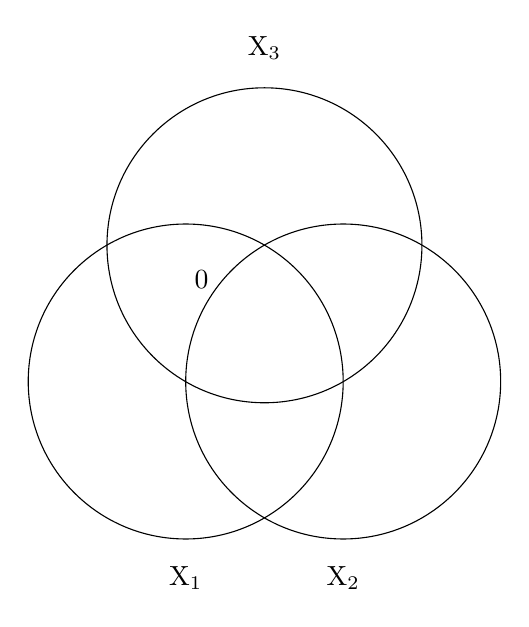
\begin{tikzpicture}
  % Draw the circles
  \draw (0,0) circle (2);
  \node at (0,-2.5) {X$_1$}; % Label below the circle for clarity
  
  \draw (2,0) circle (2);
  \node at (2,-2.5) {X$_2$}; % Label below the circle for clarity
  
  \draw (1,1.73) circle (2);
  \node at (1,4.23) {X$_3$}; % Label above the circle for clarity
  \node at (0.2, 1.3) {0};
\end{tikzpicture}
We can turn the diagram into 3 mountains now.
We can easily demonstrate with the "mountains" that $I(X_1;X_3|X_2)=0$. \\
Also $\mu^*(X_1\cap X_2\cap X_3)=\mu^*(X_1\cap X_3)$.\\
Note $\mu^*$ for a Markov chains is a measure (values are all Shannon's information measures)
\paragraph{Markov chain with 5 RVs}
5 atoms vanish.
\paragraph{Structure of $\mu^*$ for $X_1\to X_2\to X_3\to X_4$}
\[
0 = \I(X_1;X_3|X_2) = I(X_1;X_3;X_4|X_2)+I(X_1;X_3|X_2,X_4) 
\]
Let $I(X_1;X_3|X_2,X_4)=a \geq 0$. Then \[
I(X_1;X_3;X_4|X_2)=-a/
\]
By considering the subchains $X_1\to X_2\to X_4$ and $X_1\to X_3\to X_4$... we get $a=0$ so 5 atoms vanish. We can also check the non-negativity of $\mu^*$ on markov chain with 5 rvs.\\
In general, the information diagram for general markov chain can be represented by the "mountain" graph and $\mu^*$ is a measure.
\section{Information Diagram Applications}
\begin{itemize}
    \item To obtain information identities is WYSIWYG What you see is what you get.
    \item To obtain information inequalities:\begin{itemize}
        \item If $\mu^*$ is nonnegative, then $A\subset B\implies \mu^*(A)\leq \mu^*(B)$.
        \item If $\mu^*$ is a signed measure, then it's more complicated to compare $\mu^*(A)$ and $\mu^*(B)$.
    \end{itemize}
\end{itemize}
\begin{pbox}{Concavity of Entropy}
    Let $X_1\sim p_1$ and $X_2\sim p_2$, and let $X$ be a convex combination of them. Show that $H(X)
    \geq \lambda H(X_1) + \hat{\lambda}H(X_2)$.
    \newline
    Let $Z$ be a random variable independent of $X_1$ and $X_2$ that takes value $1$ with probability $\lambda$ and value $2$ with probability $1-\lambda$. Let $Z$ be the switch between $X_1$ and $X_2$ in $X\sim \lambda p_1(x)+\hat{\lambda}p_2(x)$. $\mu^*$ is a measure on 2 random variables $X$ and $Z$:
    \begin{align*}
        H(X)&\geq H(X|Z)\\
        &= P(Z=1)H(X|Z=1) + P(Z=2)H(X|Z=2)
        =\lambda H(X_)+\hat{\lambda}H(X_2)
    \end{align*}
    Interpretation: The entropy of a mixture of distributions is at least equal to the mixture of the corresponding entropies.
\end{pbox}
\begin{pbox}{Convexity of Mutual Information in the "channel"}
Let $(X,Y)\sim p(x,y)=p(x)p(y|x)$. Show that given $p(X)$, $I(X;Y)$ is a convex function of $p(y|x)$.
\begin{enumerate}
    \item Let $p_1(y|x)$ and $p_2(y|x)$ be 2 transition matrices representing 2 channels.
    \item Consider a system where the switch between 2 transition channels is determined by a random variable $Z$ as in the previous example where $Z$ is independent of $X$.
    \item Let $I(X;Z|Y)=a\geq 0$. Then \begin{equation*}
        I(X;Y:Z)=-a
    \end{equation*} because $I(X;Z)=0$.
    \item Then \begin{align*}
        I(X;Y)&\leq I(X;Y|Z)\\
        &= P(Z=1)I(X;Y|Z=1)+P(Z=2)I(X;Y|Z=2)
    \end{align*}
\end{enumerate}
Interpretation: For a fixed input distribution $p(x)$, the mutual information between the input and the output of the system obtained by mixing 2 channels $p_1(y|x)$ and $p_2(y|x)$ is at most the mixture of the 2 mutual informations corresponding to $p_1(y|x)$ and $p_2(y|x)$.x
\end{pbox}
\begin{pbox}{Concavity of Mutual Information in the "input"}
    Consider a system where the swtich on the 2 inputs is determined by $Z$. Then $Z\to X\to Y$ is a Markov chain.\\
    In the information diagram, we see $I(X;Y)\geq I(X;Y|Z)$ because $\mu^*$ is a measure for Markov processes.\\
    Now do the conditioning like before to finish the proof.\\
    Interpretation: For a fixed channel, by mixing the input distribution, the mutual information is at least equal to the mixture of the corresponding mutual informations.
\end{pbox}
\section{Shannon's Perfect Secrecy Theorem}
Let $X$ denote the plaintext, $Y$ the ciphertext, and $Z$ the key.
\newline
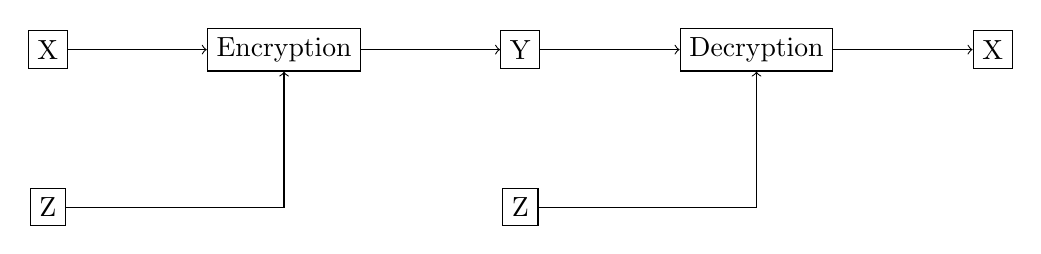
\begin{tikzpicture}[auto, node distance=2cm]
    % Nodes
    \node [draw, rectangle] (X) {X};
    \node [draw, rectangle, below of=X, node distance=2cm] (Z1) {Z};
    \node [draw, rectangle, right of=X, node distance=3cm] (encryption) {Encryption};
    \node [draw, rectangle, right of=encryption, node distance=3cm] (Y) {Y};
    \node [draw, rectangle, below of=Y, node distance=2cm] (Z2) {Z};
    \node [draw, rectangle, right of=Y, node distance=3cm] (decryption) {Decryption};
    \node [draw, rectangle, right of=decryption, node distance=3cm] (output) {X};

    % Connections
    \draw [->] (X) -- (encryption);
    \draw [->] (Z1) -| (encryption);
    \draw [->] (encryption) -- (Y);
    \draw [->] (Y) -- (decryption);
    \draw [->] (Z2) -| (decryption);
    \draw [->] (decryption) -- (output);
\end{tikzpicture}
\newline
We define perfect secrecy as \begin{equation*}
    I(X;Y)=0.
\end{equation*}
We define decipherability/correctness as \begin{equation*}
    H(X|Y,Z)=0.
\end{equation*}
These requirement implies $H(Z)\geq H(X)$, i.e., the length of the key is at least the same as the length of the plaintext (I think we should note that this is assuming uniform distribution).\\
Shannon (1949) gave a combinatorial proof.\\
We can obtain the result using information diagram:
\newline
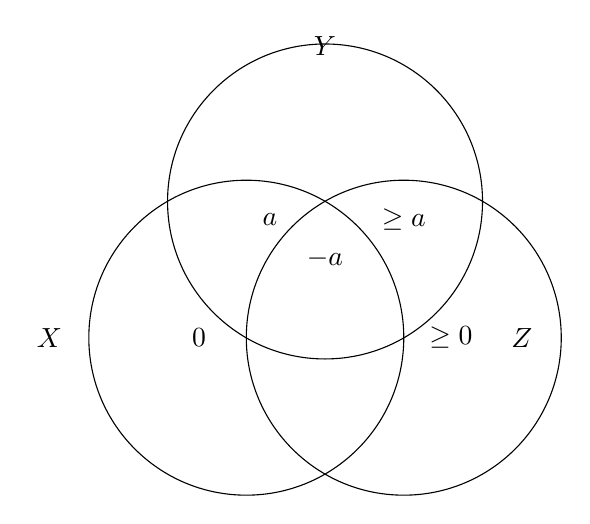
\begin{tikzpicture}
    % Draw the three circles
    \draw (0,0) circle (2cm);
    \draw (2,0) circle (2cm);
    \draw (1,1.73) circle (2cm);

    % Labels for the circles
    \node at (-2.5,0) {$X$};
    \node at (3.5,0) {$Z$};
    \node at (1,3.7) {$Y$};

    % Intersection labels
    \node at (1,1) {$-a$};
    \node at (-0.6,0) {$0$};
    \node at (2.6,0) {$\ge 0$};
    \node at (0.3,1.5) {$a$};
    \node at (2,1.5) {$\ge a$};
\end{tikzpicture}
\newline
By looking at the atoms, we see that $\mu^*(Z)\geq \mu^*(X)$
\begin{pbox}{Example: Imperfect Secrecy Theorem}
    Since $X$ can be recovered from $Y$ and $Z$, we have $H(X|Y,Z)=0$. Show that this constraint implies $I(X;Y)\geq H(X)-H(Z)$.\\
    Interpretation: $I(X;Y)$ measures the "leakage of information." When $I(X;Y)=0,$ it reduces to Shannon's perfect secrecy theorem.\\
    Fangyuan: I drew the diagram on paper and saw that this is true.
\end{pbox}
\begin{pbox}{Example: Data Processing Theorem}
    This theorem can be visualized using the information diagram, providing a more enlightening proof.
\end{pbox}
\begin{remark}
    Many identities and equalities are difficult to discover without an information diagram. 
\end{remark}
Note Shannon's information inequalities implied by basic inequalities can be verified by ITIP. The system returns ture/false/not provable.



\chapter{Zero-Error Data Compression} 
\section{The Entropy Bound}
In this section, we study why entropy is a fundamental bound for how much we can compress data.
\begin{gbox}{D-ary Source Code}
    A D-ary source code $\C$ for a source random variable $X$ is a mapping from the alphabet of $\X\to D^*$, the set of all finite length sequences of symbols taken from a $D$-ary code alphabet.
\end{gbox}
\begin{gbox}{Decodability}
    A code $\C$ is uniquely decodable if for any finite source sequence, the sequence of code symbols corresponding to this source sequence is different from the sequence of code symbols corresponding to any other finite source sequence.
\end{gbox}
\begin{pbox}{An example of source code}
    Let $\X$ be $\{A,B,C,D\}$. Consider the code $\C$ defined by \begin{align*}
        \C(A)=0\\
        \C(B)=1\\
        \C(C)=01\\
        \C(D)=10
    \end{align*}
    For example, \begin{itemize}
        \item $x=B$ is a source symbol
        \item AAD is source sequence
        \item The mapping $\C(X)$ is a source code
        \item $0010$ is a code sequence
    \end{itemize}
Note $AAD\to 0010$, $ACA\to 0010, AABA\to 0010$, so the source code $\C$ is not uniquely decodable because given a code sequence, we cannot certainly recover the source sequence.
\end{pbox}
\begin{bbox}{Kraft Inequality}
Let $\C$ be a D-ary source code, and let $l_1,l_2,\dots,l_m$ be the lengths of the codewords. If $\C$ is \textbf{uniquely decodable}, then \begin{equation*}
    \sum_{k=1}^{m}D^{-l_k} \leq 1.
\end{equation*}    
\begin{pbox}{Proof Technique}
    Consider the code $\C$ in the previous example. Let $l_1=l_2=1$ and $l_3=l_4=2$. These correspond to the lengths of the codewords in $\C$.\\
    Consider the polynomial $\sum_{k=1}^{4}2^{-l_k}=2^{-1}+2^{-1}+2^{-2}+2^{-2}$.\\
    If we raise the polynomial to the power 2 (this is a combinatorial argument. Think of each source symbol as a term in the polynomial and it quickly makes sense): \begin{align*}
        &(2^{-1}+2^{-1}+2^{-2}+2^{-2})^2\\
        &= 4\cdot 2^{-2} + 8\cdot 2^{-3} + 4\cdot 2^{-4}\\
        &=A_1\cdot 2^{-2} + A_2\cdot 2^{-3} + A_3\cdot 2^{-4}
    \end{align*}
    Then $A_2=4$ is the total number of sequences of $N=2$ codewords with a toal length of 2 code symbols: $00(AA), 01(AB), 10(BA), 11(BB).$
    Similarly, $A_3=8$ is the total number of sequnces of 2 codewords with a total length of 3 code symbols.
\end{pbox}
\begin{proof}
    Without loss of generality, assume $l_1\leq l_2\leq\dots\leq l_m$.\\
    Let $N$ be an arbitrary positive integer, and consider \begin{align*}
        &(\sum_{k=1}^{m}D^{-l_k})^N\\
        &= \sum_{k_1}^m\sum_{k_2=1}^{m}\dots\sum_{k_N=1}^{m}D^{-(l_{k_1}+\dots+l_{k_N})} \hspace{5mm} \text{typical power of sum expansion}
    \end{align*}
    Next, express as \begin{align*}
        &(\sum_{k=1}^{m}D^{-l_k})^N = \sum_{i=1}^{N\cdot l_m}A_i D^{-i}
    \end{align*}
    Now note that $A_i$ gives the total number of sequences of $N$ codewords with a total length of $i$ code symbols. (generalization of the example above).\\
    Next, since the code is uniquely decodable, these code sequences must be distinct, and therefore \begin{equation*}
        A_i\leq D^{i}
    \end{equation*}
    because there are $D^i$ distinct sequences of $i$ code symbols.\\
    Then $(\sum_{k=1}^{m}D^{-l_k})^N\leq N\cdot l_m$.\\
    Then $\sum_{k=1}^{m}D^{-l_k}\leq (N\cdot l_m)^{1/N}$ for any $N$. We obtain the inequality by letting $N\to \infty$ (the limit is the empty product $1$, the log argument).\\
    (There's an interesting proof without heavy machinary that uses the inequality $n^{\frac{1}{n}}\leq 1+2\sqrt{\frac{1}{n}}$, though this inequality is hard to discover.)
\end{proof}
\end{bbox}

\subsection{Expected Length of code}
    \begin{remark}
        Source code in information theory is not the same as source code in software engineering. In information theory, source is a random variable, code is a mapping from the alphabet of source to some representations of the letters. In software enginnering, source code is the code a programmer writes.
    \end{remark}
    Let $X\sim \{p_1,\cdots,p_m\}$.\\
    The expected length of $\C$ is: \begin{equation*}
        L=\sum_{i}p_il_i
    \end{equation*}\\
    Intuitively, for a uniquely decodable code $\C$, \begin{equation*}
        H_D(X)\leq L
    \end{equation*} because for $X$ to be recoverable, and each $D-ary$ symbol can carry at most one $|D|$-it of information.
    \begin{bbox}{Entropy Bound}
        Let $\C$ be a D-ary \textbf{uniquely decodable code} for a source random variable $X$ with entropy $H_D(X)$. Then the expected length of $\C$ is lower bounded by $H_D(X)$:\begin{equation*}
            L\geq H_D(X).
        \end{equation*}
        This lower bound is tight if and only if $l_i = -\log_D p_i$ for all $i$.
        \begin{proof}
            Since $\C$ is uniquely decodable, the lengths of the codewords satisfy the kraft inequality. \begin{align*}
                L=\sum_i p_il_i=\sum_ip_i\log_D D^{l_i}
            \end{align*}
            Recall that \begin{equation*}
                H_D(X)=-\sum_ip_i\log_D p_i
            \end{equation*}
            Then \begin{align*}
                &L-H_D(X)=\sum_ip_i(\log_Dp_i+\log_DD^{l_i})\\
                &=\sum_ip_i\log_D(p_i\times D^{l_i})\\
                &=(\ln D)^{-1}\sum_ip_i\ln(p_i\times D^{l_i})\\
                &\geq (\ln D)^{-1}\sum_i p_i (1-\frac{1}{p_iD^{l_i}})\hspace{5mm} \text{by the fundamental inequality}\\
                &= (\ln D)^{-1}\sum_i (p_i-D^{-l_i})\\
                &= (\ln D)^{-1}\left[ 1-\sum_i (-D^{-l_i})\right]\\
                &\geq (\ln D)^{-1}(1-1)\\
                &=0
            \end{align*}
            In order to achieve equality, we need equality in the fundamental inequality: $p_iD^{l_i}=1$, so $l_i=-\log_Dp_i$. If this is true, then \begin{equation*}
                \sum_iD^{-l_i} = \sum_i p_i = 1,
            \end{equation*} so the kraft inequality is also tight, automatically.
        \end{proof}
        \begin{corollary*}
            \begin{equation*}
                H(X)\leq \log|X|.
            \end{equation*} 
            We proved this earlier. The idea is to have a random variable and we represent the its source symbols by themselves (an $|\X|$-ary code). Here $L=1$ and \[
            1=L\geq H_{|\X|}(X)
            \]. We get the result through a change of basis.
        \end{corollary*}
    \end{bbox}
    \begin{gbox}{Redundancy of a coe}
        The redundancy $R$ of a $D$-ary uniquely decodable code is the difference between the expected length of the code and the entropy of the source.\begin{equation*}
            R=L-H_D(X)\geq 0.
        \end{equation*}
    \end{gbox}
\section{Prefix Codes}
Prefix code is a very important class of uniquely decodable codes.
\begin{gbox}{Prefix-free code}
    A code is called a prefix-free code if no codeword is a prefix of any other codeword. \\
    (For brevity, a prefix-free code is called a prefix code.lol )
    \begin{pbox}{Example}
        \begin{align*}
            \C(A)=0\\
            \C(B)=10\\
            \C(C)=110\\
            \C(D)=1111
        \end{align*}
        Here $\C$ is a prefix-code.
    \end{pbox}
\end{gbox}
\centering{\textbf{Code Tree for Prefix Code}}
\begin{itemize}
    \item The tree representation of a prefix code is called a code tree.
    \item A D-ary tree is a graphical representation of a collection of finite sequences of $D$-ary symbols.
    \item A node is either an internal node or a leaf.
\end{itemize}
\centering{\textbf{Instantaneous Decoding}}
The the code $\C$ in the previous example (the pink box above), we see that 
\[
BCDAC\dots \to 1011011110110\dots
\]
When we concatenate the codewords, their boundaries are not clear.\\
The stream of coded symbols are then transmitted to the receiver. \\
Since $\C$ is a prefix code, the codewords can be represented by a code tree!

\begin{tikzpicture}
    % Root node
    \node (root) at (0,0) {};
    
    % Branches and nodes
    \node (node0) at (1,-1) {};
    \node (node10) at (2,-2) {};
    \node (node110) at (3,-3) {};
    \node (node1111) at (4,-4) {};
    
    % Draw lines
    \draw (root) -- (node0);
    \draw (node0) -- (node10);
    \draw (node10) -- (node110);
    \draw (node110) -- (node1111);
    
    % Dots at nodes
    \fill (root) circle (2pt);
    \fill (node0) circle (2pt);
    \fill (node10) circle (2pt);
    \fill (node110) circle (2pt);
    \fill (node1111) circle (2pt);
    
    % Labels
    \node[above left] at (1.5,-0.5) {$0$};
    \node[above left] at (2.5,-1.5) {$10$};
    \node[above left] at (3.5,-2.5) {$110$};
    \node[above left] at (4.5,-3.5) {$1111$};
    
    % Side labels
    \node[left] at (-0.5,0) {$0$};
    \node[left] at (-0.5,-1) {$1$};
    \node[left] at (-0.5,-0.5) {$\uparrow$};
    \node[left] at (-0.5,-1.5) {$\downarrow$};
    
\end{tikzpicture}\\
Convention: Going up is 0 and going down is 1.\\
Instanteneous decoding: tracing the code tree from the root: \begin{equation*}
    1011011110110 \to 10, 110,...
\end{equation*}
First, we receive a $1$, so starting at the root, we need to go down, then we see a $0$, and we found a node that matches the code so far (10). For 110, restarting from the root, we see a 1, so go down, then another 1, then go down, then we see a 0, we enter the branch and get $110$.\\
We say that prefix codes are self-punctuating.
\begin{bbox}{Existance of prefix-code}
    There exists a $D-ary$ prefix code with codeword lengths $l_1,\dots,l_m$ if and only if the krafy inequality \begin{equation*}
        \sum_{k=1}^{m} D^{-l_k} \leq 1
    \end{equation*} is satisfied.
    \begin{proof}
        For the forward direction, we saw from the above algorithm that a prefix-code is uniquely decodable and hence satisfies Krafy inequality. \\
        For the backward direction, assume WLOG $l_1\leq \dots\leq l_m$. Consider all the D-ary sequences of lengths less than or equal to $l_m$ and regard them as the nodes of the D-ary tree of depth $l_m$. We will refer to sequence of lenfth $l$ as a node of order $l$. There are $D^{l_1}>1$ nodes of order $l_1$ can can be chosen as the first codeword. Thus choosing the first codeword is always possible. Assume that the first $i$ codewordss have been chosen successfully where $1\leq i\leq m-1$ and we want to choose a node of order $l{i+1}$ as the $(i+1)$th codeword such that it is not prefixed by any of the previous chosen codewords.\\
        Since all the previously chosen codewords are not prefixes of each other, their decendants of order $l_{i+1}$ do not overlap. The $(i+1)$th node that we choose cannot be a secendant of any of the previously chosen codeword. For node of depth $n$, the number of descendants of order $l_{i+1}$ is $D^{l_{i+1}-l_n}$. \\
        Therefore the number of nodes which can be chosen as the $(i+1)$th codeword is \[
        D^{l_{i+1}}-\sum_{k=1}^iD^{l_{i+1}-l_k}
        \]
        If $l_1,...,l_m$ satisfy the kraft inequality, we have $D^{-l_1}+\dots + D^{l_{i+1}}\leq 1$.\\ 
        Multuply by $D^{l_{i+1}}$ we get 
        \[
        \sum_{k=1}^{i+1}D^{l_{i+1}-l_k}\leq D^{i_{i+1}},
        \]
        which implies \[
        D^{l_{i+1}}-D^{l_{i+1}-l_1}-\dots -D^{l_{i+1}-l_i}\geq 1
        \]
        meaning a choice exists, so by induction, a prefix code exists.
    \end{proof}
\end{bbox}
\subsection{D-adic Distributions}
\begin{gbox}{D-adic Distributions}
    Let $p_i=D^{-t_i}$ for a;; $i$, where $t_i$ is an integer.\\
    This is called a dyadic distribution when $D=2$.
    \begin{corollary*}
        There exists a D-ary prefix code which achieves the entropy bound for a distribution $\{p_i\}$ if and only if $\{p_i\}$ is D-adic.
    \end{corollary*}
    \begin{proof}
        Consider a D-ary prefix code which achieves the entropy bound for a distribution $\{p_i\}$. Let $l_i$ be the length of the codeword assigned to the probability $p_i$. Then by the entropy bound, $l_i=-\log_D p_i$ (condition for entropy bound to be tight), or\begin{equation*}
            p_i = D^{-l_i}.
        \end{equation*}
        This $\{p_i\}$ is D-adic.\\
        For the if direction: suppose $\{p_i\}$ is D-adic, then $t_i=-\log_D p_i$. Let $l_i=t_i$ for all $i$. verify that $\{l_i\}$ satisfies the Kraft inequality:\[
        \sum_i D_{l_i} = \sum_i p_i =1\leq 1.
        \]
        Then there exists a prefix code with codeword lengths $l_i$'s. Assign the codeword with length $l_i$ the probability $p_i$. 
    \end{proof}
\end{gbox}
\end{document}